\documentclass[11pt,a4paper]{article}

\usepackage[a4paper,margin=25mm]{geometry}
\usepackage[T1]{fontenc}
\usepackage[utf8]{inputenc}
\usepackage[british]{babel}
\usepackage{newtxtext,newtxmath}
\usepackage{microtype}
\usepackage{setspace}
\setstretch{1.16}
\usepackage{amsmath,bm}
\usepackage{booktabs,longtable,tabularx,array,ragged2e,multirow}
\usepackage{graphicx}
\graphicspath{{figures/}}
\usepackage{caption}
\captionsetup{font=small,labelfont=bf,labelsep=period,justification=justified,singlelinecheck=false}
\usepackage{float}
\usepackage{enumitem}
\setlist{leftmargin=1.5em,itemsep=0.15em,topsep=0.3em}
\usepackage{xcolor}
\definecolor{ink}{HTML}{252B25}
\definecolor{muted}{HTML}{596052}
\usepackage{titlesec}
\titleformat{\section}{\large\bfseries\color{ink}}{\thesection}{0.7em}{}
\titleformat{\subsection}{\normalsize\bfseries\color{ink}}{\thesubsection}{0.7em}{}
\titleformat{\subsubsection}{\normalsize\bfseries\color{ink}}{\thesubsubsection}{0.6em}{}
\titlespacing*{\section}{0pt}{1.5ex plus .3ex}{0.7ex}
\titlespacing*{\subsection}{0pt}{1.2ex plus .2ex}{0.5ex}
\usepackage[numbers,sort&compress]{natbib}
\usepackage[colorlinks=true,linkcolor=black,citecolor=black,urlcolor=black]{hyperref}
\usepackage[nameinlink,noabbrev,capitalize]{cleveref}
\usepackage{lineno}
\modulolinenumbers[1]
\renewcommand\linenumberfont{\normalfont\scriptsize\sffamily\color{muted}}
\setlength{\parindent}{1.2em}
\setlength{\parskip}{0pt}
\setlength{\emergencystretch}{2em}
\setlength{\tabcolsep}{4pt}
\renewcommand{\arraystretch}{1.12}
\newcolumntype{L}[1]{>{\RaggedRight\arraybackslash}p{#1}}
\newcommand{\vect}[1]{\bm{#1}}
\newcommand{\Ecc}{E_{\mathrm{cc}}}

\title{\textbf{From routine cine CMR to regional myocardial dysfunction:}\\
\large Fidelity, validation and interpretation of motion and strain estimates}
\author{Ziying Huo\\[0.25em]
\small Faculty of Biology, Medicine and Health, The University of Manchester, Manchester, United Kingdom\\
\small ORCID: \href{https://orcid.org/0009-0003-1090-8784}{0009-0003-1090-8784}\\
\small Correspondence: \href{mailto:ziying.huo@postgrad.manchester.ac.uk}{ziying.huo@postgrad.manchester.ac.uk}\\
\small Full postal correspondence address to be confirmed before submission}
\date{8 October 2026}

\begin{document}
\linenumbers
\maketitle
\begin{center}
\small Article type: Review
\end{center}

\begin{abstract}
Regional myocardial dysfunction can be clinically important while global ventricular measures remain preserved. Routine cine cardiovascular magnetic resonance (CMR) is widely available and supports retrospective motion and strain estimation, and what it records is changing image intensity and anatomy without labels for myocardial material points. Every estimator therefore adds assumptions to recover correspondence, and the question for a regional claim is which attributes of an abnormality, its magnitude, location, spatial extent and timing, are recovered within a tolerance appropriate to the intended use.

This critical narrative review compares feature-tracking, deformable-registration, biomechanical and learning-based estimators by their inputs, representations, priors and supervision, and groups the validation literature by the claim each target can support: numerical phantoms, tagging, displacement encoding with stimulated echoes (DENSE), scan--rescan studies, late gadolinium enhancement and clinical outcomes. Current evidence most directly supports cine-derived circumferential strain at whole-slice, global and segmental scales under matched definitions, including improved segmental agreement with DENSE after DENSE-supervised learning. Agreement is weaker for regional than global quantities and weakest for radial strain. The one independent test against a prescribed focal scar preserved slice-averaged circumferential strain better than radial strain without quantifying recovery of the scar region, and direct tests of focal boundary, extent and peak timing remain sparse.

Apparent contradictions resolve when representation capacity, estimation error and input sufficiency are separated and when estimands are matched. A defensible validation programme pre-specifies the measurement contract, combines known-motion tests with registered material-sensitive in-vivo comparisons, and ties each regional claim to the method, acquisition, population, scale and reference for which it was demonstrated.
\end{abstract}

\noindent\textbf{Keywords:} cardiovascular magnetic resonance; cine CMR; myocardial motion; myocardial strain; regional dysfunction; feature tracking; image registration; validation.

\section*{Plain English summary}
The heart can contain a small area that moves abnormally even when its overall pumping measure looks normal. Standard cine CMR provides moving pictures of the heart and is available in routine care. Computer methods can use these pictures to estimate motion and strain, a measure of deformation. An ordinary cine image, however, does not label each piece of heart muscle, so different methods can produce different internal motion while matching the same heart borders.

We reviewed how cine-based methods work and how they have been tested. Some studies show useful agreement with specialised CMR methods that are more sensitive to tissue motion. Other studies show important differences between software products, strain directions and heart regions. A good-looking contour, a repeatable number, an association with scar and a prediction of outcome are all valuable findings, and each of them proves a different thing.

Regional measurements should therefore be judged for the exact property they are meant to report: the size, position, extent or timing of an abnormality. Tests with known motion should be combined with carefully registered comparisons to specialised scans in people. The method, scan settings, strain definition and acceptable error should be stated in advance. This approach can identify where routine cine CMR gives reliable regional information and where the result should remain qualified.

\section{Why regional function is a distinct measurement problem}

Left-ventricular ejection fraction compresses a complex three-dimensional deformation into a chamber-level ratio. That compression is valuable: ventricular volumes and ejection fraction are reproducible CMR endpoints, widely understood and embedded in clinical reporting standards\cite{schulzmenger2020,hundley2022}. It is nevertheless possible for well-functioning regions to compensate for a smaller abnormal region, for opposing changes to cancel in an average, or for the timing of regional contraction to change without a large fall in ejection fraction. Regional motion and strain are therefore attractive when the clinical question concerns focal infarction, heterogeneous cardiomyopathy, dyssynchrony, early dysfunction or treatment response.

Clinical studies support the relevance of myocardial deformation. Feature-tracking strain has been associated with functional recovery after myocardial infarction, adverse remodelling and cardiovascular outcomes\cite{buss2015,reindl2021,chadalavada2024}; DENSE circumferential strain has also shown prognostic association after acute infarction\cite{mangion2019}. These observations justify measuring deformation, but they do not settle how accurately a regional abnormality has been located or quantified. A prognostic marker can remain useful despite measurement bias, and a technically accurate motion field may not improve a clinical decision. Analytical validity, biological association and clinical utility are linked but separate questions\cite{raunig2015,puntmann2018}.

Several reviews have described strain physics, modality differences, clinical practice and sources of discrepancy\cite{amzulescu2019,smiseth2025}. More recent reviews cover deep learning for wall-motion analysis across modalities and strain from CMR and computed tomography\cite{monfared2026review,hussein2026review}. The present review has a narrower purpose. It asks how faithfully routine cine CMR can recover \emph{regional or focal} myocardial dysfunction, and how a validation target changes the claim that can be made. The emphasis is not a contest between named algorithms. It is a comparison of their inputs, assumptions, estimands, populations and reference standards.

The practical question is:

\begin{quote}
For a specified cine acquisition, estimator and measurement definition, which attributes of a regional abnormality---magnitude, location, spatial extent and timing---are recovered within a tolerance that is appropriate for the intended use?
\end{quote}

This formulation avoids two unhelpful extremes. Routine cine is not information-free: myocardial borders, papillary muscles, trabeculation, intensity variation, neighbouring structures and temporal consistency all constrain motion. Conversely, a visually plausible deformation or accurate contour does not uniquely identify how material points moved within the myocardium. The evidence supports bounded successes rather than a universal verdict.

\subsection{Review approach and scope}

This is a critical narrative review, not a systematic review or meta-analysis. The inherited historical search used 18 query--database combinations with a 1 September 2026 cutoff: 281 exported rows became 253 unique candidates, from which 21 records were retained; a 9 September top-up produced a final near-neighbour matrix of 23 records representing 22 studies. It was one AI-assisted screening stream, without independent duplicate screening or a full-text exclusion stage. A separate supplied set of 42 auxiliary research leads and a targeted verification update through 8 October 2026 were used to check central primary studies, resource metadata, recent publication status and adjacent reviews; they are not added to the historical denominator. PubMed/PMC, publisher pages, Crossref/DataCite metadata and official dataset or journal pages were prioritised. Where only an abstract was inspected, the manuscript uses only abstract-level claims. Search boundaries, source URLs and reading depth are recorded in the accompanying evidence ledger and Supplementary Methods.

Studies were compared along six axes: (1) image input and sampling; (2) population and abnormality; (3) estimated entity, such as contour motion or dense displacement; (4) strain definition and aggregation; (5) validation target; and (6) reported error or association. Results were not pooled because these axes, reference standards and endpoints were too heterogeneous. Dice overlap, displacement error, strain bias, scan--rescan precision, scar discrimination and outcome association were treated as different quantities rather than placed on a common performance scale.

\section{From cine images to a regional measurement}

\subsection{What routine cine CMR observes}

Balanced steady-state free-precession cine CMR samples a time series of image intensities. In a typical short-axis image, the blood--myocardium interfaces are conspicuous, whereas intramyocardial texture can be weak and changes with coil sensitivity, through-plane motion, partial volume, reconstruction and artefact. The image therefore supplies anatomical and intensity cues, not a persistent identity label for every tissue element. Feature tracking exploits image features or propagated contours; registration exploits an image-similarity relation; biomechanical models constrain admissible deformation; and learning-based methods import associations learned from training data\cite{pedrizzetti2016,duchateau2020}. These categories overlap. A neural network may predict registration parameters, a registration method may use a learned similarity measure, and a biomechanical penalty may be embedded in either.

\begin{figure}[H]
\centering
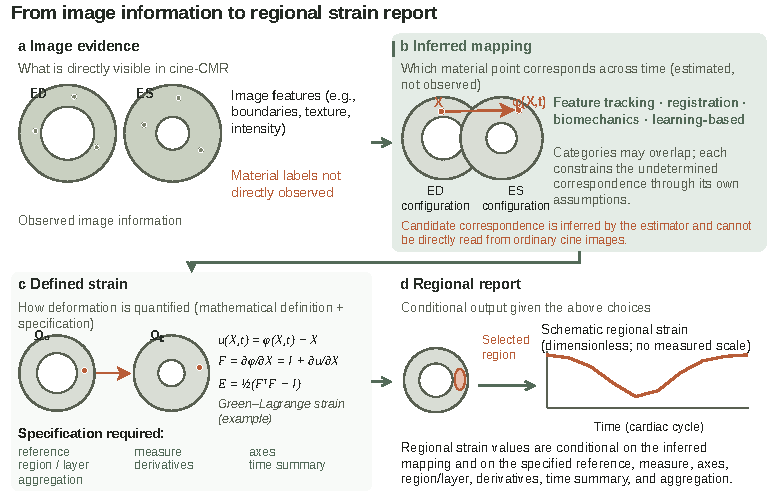
\includegraphics[width=\textwidth]{Figure_1_image_to_regional_report.pdf}
\caption{From image information to a regional strain report. Routine cine directly contains time-varying anatomy and image cues (a), whereas material correspondence is inferred by an estimator (b). A deformation measure is then defined from the mapping and a complete measurement specification (c) before regional aggregation or time summarisation (d). The curve is a dimensionless schematic with no measured scale. All elements are original deterministic vector schematics; no patient image or experimental result is shown. OpenAI Codex (gpt-5.6-sol) assisted deterministic Draw.io XML and Python-builder edits; no generative image model was used. Author verification is required before submission.}
\label{fig:image-to-report}
\end{figure}

The distinction in \cref{fig:image-to-report} is causal, not semantic. Let a point in a reference configuration be \(\vect X\), and let an estimated mapping be \(\boldsymbol\varphi(\vect X,t)\). The displacement and deformation gradient are
\begin{equation}
\vect u(\vect X,t)=\boldsymbol\varphi(\vect X,t)-\vect X,
\qquad
\vect F(\vect X,t)=\frac{\partial\boldsymbol\varphi}{\partial\vect X}
=\vect I+\frac{\partial\vect u}{\partial\vect X}.
\end{equation}
One possible finite-strain measure is the Green--Lagrange tensor,
\begin{equation}
\vect E=\frac{1}{2}(\vect F^{\mathsf T}\vect F-\vect I).
\end{equation}
The equations do not guarantee that \(\boldsymbol\varphi\) is correct. They state how a chosen mapping is converted into a chosen strain. Differentiation can amplify local mapping error, while smoothing can reduce variance and alter peaks or spatial gradients. The reported number further depends on coordinate axes, myocardial layer, reference frame, segment definition, spatial aggregation and whether ``peak'' means the minimum of a segment-average curve or the average of pointwise minima. Comparisons that ignore these choices can attribute a definitional difference to a tracking error\cite{voigt2015,wehner2018}.

\subsection{The same contours can support different material mappings}

Boundary agreement constrains deformation but does not determine it. Consider an annulus whose end-diastolic and end-systolic contours are fixed. Material points can retain their angular positions or be reparameterised around the same final contour. Both mappings have Dice overlap of one and Hausdorff distance of zero for the masks, yet their circumferential stretch varies differently with position (\cref{fig:same-contours}). This counterexample proves a limited but important point: equal masks or equal mean geometry are insufficient to identify intramyocardial correspondence. It does not prove that cine-derived regional strain is always wrong, nor that image texture and temporal information cannot select a useful mapping.

\begin{figure}[H]
\centering
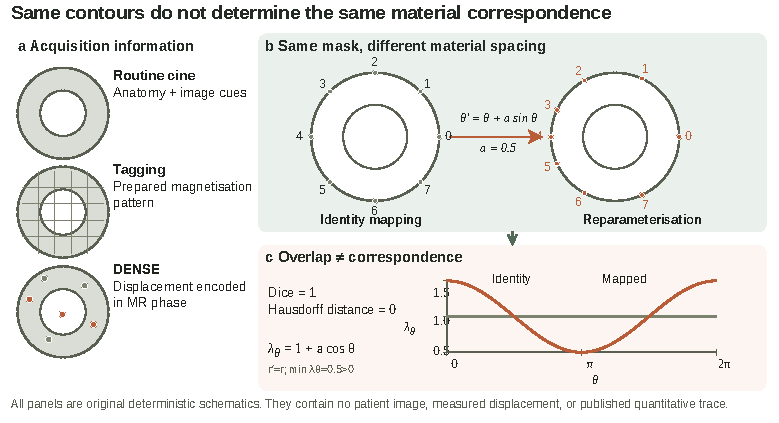
\includegraphics[width=\textwidth]{Figure_2_same_contours_not_same_correspondence.pdf}
\caption{Same contours do not determine the same material correspondence. Panel a contrasts, schematically, the information supplied by routine cine, tagging and DENSE. Panel b shows two possible correspondences between identical annular contours. Panel c uses the declared analytic example \(r'=r\), \(\theta'=\theta+a\sin\theta\), with \(a=0.5\). Its circumferential stretch is \(\lambda_\theta=1+a\cos\theta\), ranging from 0.5 to 1.5; orientation is preserved for \(|a|<1\). Both mappings have identical annular masks, but different material-point correspondence. This is an analytic counterexample, not a measured cardiac result. OpenAI Codex (gpt-5.6-sol) assisted deterministic Draw.io XML and Python-builder edits; no generative image model was used. Author verification is required before submission.}
\label{fig:same-contours}
\end{figure}

This non-uniqueness matters most as the claim becomes more local. Chamber volume can be estimated from boundaries. A global contour-length change is also strongly boundary-constrained. A segmental average requires correspondence between sectors. Transmural or voxelwise strain additionally requires intramyocardial correspondence and spatial derivatives. Thus, a method can be accurate for volumes and useful for global strain while remaining insufficiently validated for focal strain gradients. Validation should follow the finest claimed spatial and temporal scale rather than inherit credibility from an upstream task.

\subsection{A complete estimand is more than the word ``strain''}

At minimum, a regional strain estimand should state:

\begin{itemize}
\item the reference configuration and mapping direction;
\item the finite-strain measure (for example, linear, Green--Lagrange or logarithmic strain);
\item the anatomical coordinate system and sign convention;
\item the myocardial layer and dimensional model (2D slice, 2D+time or 3D+time);
\item the differentiation, interpolation and spatial regularisation used;
\item the region definition, registration to the AHA model and treatment of junctions;
\item the temporal summary, including end-systolic versus peak strain and handling of post-systolic shortening; and
\item the order of spatial and temporal aggregation.
\end{itemize}

Without these items, apparent disagreement may reflect different quantities. The problem is prominent for radial strain, for which wall-thickening surrogates, tensor components and layer-specific measurements are not interchangeable. It also affects circumferential comparisons when one pipeline reports one-dimensional engineering strain and another reports a component of a two-dimensional Green--Lagrange tensor\cite{wehner2018,cao2018}.

\section{Estimator families and the assumptions they contribute}\label{sec:families}

All estimators resolve incomplete image information by adding structure. The relevant comparison is therefore not ``assumption-free'' versus ``model-based'', but which assumptions are introduced, whether they are visible to the user, and whether they are appropriate for the abnormality being studied. \Cref{tab:families} summarises these attribute-level distinctions; \cref{sec:illposed} states the estimation problem they all share, and \cref{sec:ft} to \cref{sec:supervised} then follow the literature in approximate chronological order within each family. A year-ordered table of the individual methods, with the data, validation approach and pathology evaluation each source reports, is given in Supplementary Table~S3.

{\scriptsize\sloppy
\setlength{\tabcolsep}{2pt}
\begin{longtable}{L{0.09\textwidth}L{0.115\textwidth}L{0.11\textwidth}L{0.105\textwidth}L{0.115\textwidth}L{0.11\textwidth}L{0.145\textwidth}}
\caption{Method attributes that may coexist within a cine-CMR motion estimator. Rows are descriptive archetypes, not mutually exclusive method families.}\label{tab:families}\\
\toprule
Archetype & Input & Output and estimand & Motion representation & Constraint/prior & Optimisation or training target & Endpoint directly validated in representative work \\
\midrule
\endfirsthead
\toprule
Archetype & Input & Output and estimand & Motion representation & Constraint/prior & Optimisation or training target & Endpoint directly validated in representative work \\
\midrule
\endhead
Feature and contour tracking & Cine pixels plus initial contours & Contour/mesh motion; product-defined strain & Boundary points, meshes or proprietary field & Feature similarity and trajectory continuity & Frame-to-frame match or contour propagation & Global/segmental peak strain, repeatability and tissue discrimination; product-specific \\
\addlinespace
Deformable registration & Image pairs or cine sequence & Dense displacement; derived strain & Voxel field, spline, spectral or implicit field & Spatial/temporal regularity; optional topology & Image/feature similarity plus penalties & Image/shape alignment; selected phantom, tagging or DENSE comparisons \\
\addlinespace
FE model & Images, masks or meshes & Nodal displacement and tensor strain & Finite-element or reduced-order basis & Compatibility, volume constraint, constitutive/fibre terms & Image correlation plus mechanical residual & Landmark/curve or phantom error in the specified model domain \\
\addlinespace
Supervised learning & Cine or contours plus motion/strain labels & Learned displacement or strain & Dense field or parameter map & Architecture, augmentation and label domain & Label loss; optional image, shape or mechanics terms & Depends on label: StrainNet separates DENSE-contour EPE from cine-contour Ecc \\
\addlinespace
Self-supervised learning & Cine without motion labels & Dense displacement/strain & Usually voxel or multi-scale field & Smoothness, cycle, topology or shape & Image, feature or mask agreement & Commonly registration and anatomy; material endpoints require separate testing \\
\addlinespace
Compact basis & Any compatible image estimator & Coefficients decoded to motion/strain & Fourier, spline, temporal or neural basis & Band limit or basis dimension & Inherits estimator objective; may be learned & Capacity and final estimator performance are distinct endpoints \\
\bottomrule
\end{longtable}
}

\subsection{An underdetermined problem, and what the prior is doing}\label{sec:illposed}

Let \(I_t(\vect x)\) denote image intensity at position \(\vect x\) in phase \(t\), and let \(\boldsymbol\varphi_{0\rightarrow t}\) map a material point in the reference configuration to its position at \(t\). Almost every estimator reviewed below can be written as, or interpreted through, the objective
\begin{equation}
\widehat{\boldsymbol\varphi}_{0\rightarrow t}
=\arg\min_{\boldsymbol\varphi_{0\rightarrow t}}
\mathcal D\!\left(I_0,\,I_t\circ\boldsymbol\varphi_{0\rightarrow t}\right)
+\alpha\,\mathcal R(\boldsymbol\varphi_{0\rightarrow t}),
\label{eq:registration}
\end{equation}
in which \(\mathcal D\) rewards image agreement, \(\mathcal R\) encodes prior structure and \(\alpha\) sets their balance. The map is written here as a forward map on the reference domain; frameworks that optimise a backward sampling map use a different convention, and the two must not be interchanged when transformations are composed or differentiated for strain. Groupwise and sequence models optimise an analogous objective over the whole cycle at once, and learning-based methods minimise its expectation over a training set rather than solving it per case.

The difficulty is that \(\mathcal D\) alone does not identify the map. Where intramyocardial texture is weak, many fields achieve nearly the same data term while implying different displacement gradients, and the prior selects among them; \cref{fig:same-contours} is the analytic instance of this non-uniqueness. Two statements about priors are easy to conflate and are kept separate throughout this review. The first concerns what a representation can \emph{express}: strain is a spatial derivative of displacement, so a displacement field that looks smooth can still carry a rapidly varying strain, and restricting the field to a band of spatial frequencies restricts the derivatives it can represent only in a way that depends jointly on the bandwidth, the spatial scale of the abnormality and the measurement definition. The second concerns the estimation \emph{process}: even with a representation rich enough to express a focal deficit, the optimiser or network may not recover it if the image evidence is weak or the penalty \(\alpha\mathcal R\) is strong. A third factor, the information actually present in the input images, is separate again.

These three come apart in practice, and the way they come apart is the basis of an attribution experiment. Suppose a focal deficit is under-recovered. If the same estimator recovers it when \(\alpha\) is reduced, the limitation was the estimation process. If it is still under-recovered after the known deficit has been projected directly onto the estimator's function space---a cheap test that uses the known field rather than the images---the limitation lies in the representation. If neither holds, but the deficit becomes recoverable when the same motion is re-imaged at finer resolution or with added long-axis views, the limitation was the input information. Attributing an observed regional error therefore requires an experiment that holds the other two factors fixed; \cref{sec:threequestions} returns to this separation when reconciling discordant results, and the known-motion resources in \cref{sec:resources} are the setting in which it can be run.

Temporal strategy adds a further assumption. Reference-to-frame tracking keeps one reference configuration but must estimate large displacements from it; sequential tracking estimates smaller inter-frame steps but accumulates composition error and drift; groupwise methods estimate all phases jointly under whatever temporal constraint they impose\cite{metz2011,chen2024}. A periodic deformation can close perfectly at the end of the cycle and still be wrong at intermediate phases, so cycle closure is a useful constraint and a useful quality-control signal rather than proof of correct material trajectories.

\subsection{Feature tracking and contour propagation}\label{sec:ft}

Feature-tracking software is attractive because it operates on routine cine and fits existing clinical workflows. Initial contours are propagated through the cardiac cycle, after which strain may be calculated from endocardial length, a myocardial mesh or a vendor-specific deformation field; interior motion is to a large degree interpolated from boundary behaviour\cite{pedrizzetti2016}. The phrase ``feature tracking'' therefore denotes a family rather than a single measurement. Commercial implementations have differed in contour placement, transmural treatment, radial-strain calculation, temporal interpolation and user correction. Even when repeatability within a product is acceptable, values may not be interchangeable across products or software versions\cite{lim2021,militaru2021}. Automating the front end was an early application of deep learning: Vigneault and colleagues segmented the sequence with a fully convolutional network and fitted quadratic basis splines across all frames in 42 patients with hypertrophic cardiomyopathy and 21 controls\cite{vigneault2017}, and Puyol-Ant\'on and colleagues combined convolutional segmentation with subsequent feature tracking and strain calculation\cite{puyolanton2018}. In both, the learned component is the segmentation and the motion model remains a conventional tracker.

The strongest interpretation of a contour-tracking result depends on what was actually tracked. A reliable change in endocardial length can support a global or segment-level contour-derived strain under that definition. It does not automatically support transmural material strain. Conversely, methods that use internal image information should not be reduced to ``border tracking'' if their documented algorithm does more. Method descriptions and validation endpoints, rather than product category labels, should govern interpretation. One evaluation caveat applies to this whole section: segmentation can initialise the search region, define the cardiac coordinate system and, in several learning-based designs, supply an anatomical loss during training. When the same reference contours both shape the fitted transformation and provide the overlap score that assesses it, the evaluation is not independent of the fitting.

\subsection{Conventional and learned registration, and the field representation}\label{sec:registration}

Intensity-based deformable registration estimates a dense field by optimising \cref{eq:registration} directly. The free-form deformation model of Rueckert and colleagues---an affine transform plus a B-spline control lattice with a smoothness penalty---remains the reference implementation and was introduced for breast MRI rather than the heart\cite{rueckert1999}. Groupwise variants remove the dependence on an arbitrarily chosen reference frame: Metz and colleagues fitted an \(n\)D\(+t\) B-spline model to the whole dynamic sequence with spatial and temporal smoothness and an optional cyclic constraint, reporting sub-voxel accuracy on synthetic and thoracic CT data\cite{metz2011}. More recently, Chen and colleagues replaced the groupwise dissimilarity term with a locally low-rank metric, evaluated on a 20-case simulation, 100 public cine cases and 16 in-house tagging patients, and reported reduced late-diastolic drift and better correlation with tagging for radial strain in several segments than optical flow, pairwise registration, global low-rank groupwise registration and \(n\)D\(+t\) B-splines\cite{chen2024}. Anatomy-aware, pyramidal and online-adaptive methods similarly change the evidence available to the optimiser and the class of admissible fields\cite{chen2020anatomy,yu2020mpn,yu2020foal}.

The learning-based literature began by amortising \cref{eq:registration}. VoxelMorph reformulated registration as a function, parameterised by a convolutional network, that maps an image pair to a deformation field; the unsupervised training objective is the same image-matching and smoothness objective that a classical method optimises per pair, and the gain is that inference becomes a single forward pass\cite{balakrishnan2019voxelmorph}. TransMorph replaced the convolutional encoder with a hybrid Transformer--convolutional architecture and added diffeomorphic and Bayesian variants, validated on brain MRI and phantom-to-CT registration\cite{chen2022transmorph}. In this family the prior is still smoothness or diffeomorphism, now partly learned, and the reported evidence is label overlap and deformation-field regularity.

A distinct strand constrains the representation rather than the penalty. B-splines, finite-element bases, Fourier coefficients, implicit neural representations and dense voxel grids have different capacity and conditioning. Fourier-Net predicts a band-limited representation of the displacement in a low-dimensional frequency domain and recovers the full-resolution field by zero-padding and an inverse discrete Fourier transform\cite{jia2023fouriernet}; Fourier-Net+ takes band-limited representations of the images themselves as input, with cascaded and diffeomorphic variants\cite{jia2026fouriernetplus}. Band-limiting is an explicit, tunable statement about which deformations the model may output, which makes this family unusually well suited to the attribution experiment of \cref{sec:illposed}; but the bandwidth is a global property of the field, and what it implies for a focal regional strain has to be measured rather than asserted. Both are general-purpose registration networks: the evaluations in the records retrieved use registration benchmarks with overlap and regularity metrics, and Fourier-Net+'s cardiac evaluation reports registration, geometric and functional measures that do not by themselves establish regional material-strain fidelity. Within the searches recorded here, this review did not identify an evaluation of a band-limited cine estimator against a regional motion or strain reference; that is a statement about what those searches returned, not an assertion that no such study exists.

\subsection{Cardiac-specific designs: joint tasks, multiple views, meshes and time}\label{sec:cardiacspecific}

A second group builds cardiac structure into the estimator. Qin and colleagues learned motion estimation and segmentation jointly, sharing a multi-scale encoder between an unsupervised Siamese recurrent spatial-transformer branch and a segmentation branch, in 220 subjects\cite{qin2018joint}. Zheng and colleagues learned a pixel-wise ``apparent flow'' between two cine phases semi-supervised from a large unsegmented and a small expert-segmented set, then derived per-segment radius and thickness time series whose nine features classified ACDC pathology with 95\% and 94\% accuracy on the training and test sets\cite{zheng2019apparent}; the motion representation is validated there through its usefulness for a downstream label rather than against a motion reference, a pattern that recurs in \cref{sec:supervised}. Motion Pyramid Networks introduced multi-scale fused estimation with a cyclic teacher--student training procedure\cite{yu2020mpn}, and FOAL added online adaptation of a learned estimator to a new sequence at test time\cite{yu2020foal}. A 2025 semi-supervised design uses all frames of the sequence with an end-diastolic distance map weighting the loss, reporting an end-point error of 1.02~mm against 1.19~mm for a retrained RAFT baseline in an in-house set of 271 patients; its strain endpoint is global peak correlation rather than a material reference\cite{portal2025semisup}.

Multi-view and mesh-based designs target through-plane motion. MulViMotion fuses short-axis and long-axis cine in a hybrid 2D/3D network with a shape-regularisation module providing weak supervision, evaluated on 580 UK Biobank subjects\cite{meng2022mulvimotion}. DeepMesh represents the heart as a 3D mesh of endocardial and epicardial surfaces, propagates a template mesh into subject space and estimates vertex-wise displacement through a differentiable mesh-to-image rasteriser, so that vertex correspondence is maintained across frames and subjects\cite{meng2024deepmesh}. CardioMorphNet takes the shape idea further: a recurrent variational autoencoder with separate posteriors for segmentation and motion, trained by recursively registering segmentation maps without an intensity-based similarity loss, validated on UK Biobank and M\&Ms by comparing warped masks with reference masks and yielding voxel-wise uncertainty maps\cite{movahed2026cardiomorphnet}. Predictive uncertainty and accurate warped masks are valuable, but uncertainty is not automatically calibrated regional error, and a Bayesian output is not automatically an abstention policy. STCMT-Net represents cardiac motion through keypoints extracted without supervision and reconstructs the dense field as a weighted combination of basis vectors from matched keypoint pairs, evaluated on 4D CT and cine MRI with a strain analysis reported to separate patients under different conditions\cite{qiao2026stcmt}.

Temporal structure has been addressed in parallel: a low-rank groupwise deformation model for cine tracking in a preprint that is a master's thesis and has not been peer reviewed\cite{rendell2024lowrank}, a Mamba-based sequential model presented in a MICCAI workshop\cite{yin2025mcm}, and a continuous-time latent neural ordinary differential equation with bidirectional forward--backward evolution and a Lagrangian consistency term, evaluated on ACDC and M\&Ms\cite{ruan2026latentode}. One parallel development belongs here because it is \emph{not} a motion-estimation development: CMR-specific foundation models now exist, one pre-trained on 15 million cine images from 74,916 studies\cite{fu2026cinema} and another trained by self-distillation on 36 million images from 27,524 subjects\cite{jacob2025cmrfm}, each fine-tuned for segmentation, landmark localisation, diagnosis and related tasks. Dense motion estimation is not among the tasks either reports, so the pre-trained representations they offer have not yet been tested on the problem this review is about.

Read together, this group has made real progress on three-dimensional motion from two-dimensional acquisitions and on temporal consistency across the cycle. Its reported validation needs stating plainly: in the cardiac-specific papers reviewed here, the dominant evidence is agreement between a warped segmentation and a reference segmentation, together with surface distances and deformation-field regularity, with landmark error where a landmarked dataset was available. That is appropriate evidence for the claims those papers make, and it is also the evidence that \cref{fig:same-contours} shows cannot by itself establish material correspondence.

\subsection{Biomechanical and physics-informed regularisation}\label{sec:physics}

A third group replaces a generic smoothness penalty with a statement about tissue mechanics or about the function space itself. Qin and colleagues learned the prior instead of writing it down: a variational autoencoder trained on biomechanically simulated deformations defines a manifold of plausible fields, and tracking becomes a search over that manifold, validated on three public cine datasets\cite{qin2023biomech}. WarpPINN states the physics explicitly, representing the deformation with a neural network fitted per case under an intensity-similarity term plus a hyperelastic regulariser and a Jacobian penalty for near-incompressibility, with strain by automatic differentiation and Fourier feature mappings to allow sharp features in the strain field; it was tested on synthetic examples and a cine benchmark of 15 healthy volunteers\cite{arratia2023warppinn}. WarpPINN-fibers adds a fibre-stretch penalty and reported improved landmark tracking and strain-curve prediction on a synthetic phantom and the same healthy benchmark\cite{alvarez2026warppinn}. Liu and colleagues combine the mechanical and temporal arguments in a space--time finite-element correlation framework with region-specific biomechanical regularisation and a data-driven temporal decomposition; their evaluation is the most layered in this group---one synthetic dataset with ground-truth motion and strain, three public datasets with landmarks or masks and a clinical dataset with masks, against two feature-tracking and four deep-learning baselines\cite{liu2026fe}. Implicit neural representations of intramyocardial motion and strain have also been presented in the 2026 STACOM proceedings, but no abstract accompanies the record retrieved, so that study is not characterised here\cite{bell2026inr}.

Such results show that mechanics can be useful inductive structure. They do not imply that a constrained field is uniquely correct: disease can alter wall thickness, loading, scar mechanics and fibre organisation, while a 2D slice omits through-plane motion. The limiting factor is the same throughout the group: where a strain reference exists at all, it exists in one simulation setting, and the in-vivo evaluation returns to landmarks and masks. A mechanical prior is not a weaker constraint than a smoothness prior, merely a differently shaped one, and whether it preserves a focal deficit depends on whether its constitutive assumptions hold in heterogeneous injured tissue---an open question rather than a defect. Validation must test whether the constraint preserves the abnormality of interest instead of evaluating plausibility alone.

\subsection{Learning from cine, contours or motion-encoded CMR}\label{sec:supervised}

The final group changes the supervision rather than the prior, and learning-based methods differ most importantly in their target. DeepTag estimates motion on tagged images without labels, using bidirectional diffeomorphic registration between consecutive frames and a differentiable composition layer to recover the Lagrangian field, validated by landmark tracking on a clinical tagging dataset\cite{ye2021deeptag}. Networks trained on synthetic 3D tagged images from a biophysical left-ventricular model have since been proposed for 3D tagging analysis\cite{buoso2025tagging3d}; like DeepTag, these operate on the comparator acquisition rather than on cine. DeepStrain is the most completely documented end-to-end cine workflow: it centres the ventricle, segments anatomy, estimates end-diastole-to-phase displacement and derives Green--Lagrange radial and circumferential strain, with the original study reporting a CMAC landmark end-point error of \(2.9\pm1.5\)~mm together with scan--rescan repeatability in ten healthy volunteers and high agreement for volumetric measures\cite{morales2021}. A later single-centre comparison in 47 healthy participants and 533 patients found correlations with manual feature-tracking analysis of 0.83--0.85 for global radial and 0.88--0.91 for global circumferential strain\cite{morales2022comparison}; the comparator is another estimator rather than a motion reference. These results establish workflow and output properties but do not, by themselves, provide independent dense material truth for the cine motion field; the independent prescribed-motion test of DeepStrain is discussed in \cref{sec:knownmotion}.

StrainNet is particularly relevant because DENSE phase-derived displacement was the supervised target, but its two evaluations must be separated. Of 305 eligible individuals (161 patients, 99 healthy adults and 45 healthy children or adolescents), 243 individuals contributing 670 sections formed the training set and 62 individuals contributing 190 sections formed the independent test set; the 305 were not independent held-out cine tests. For pixelwise displacement end-point error (EPE), the model was deliberately given contours derived from DENSE magnitude images, permitting one-to-one comparison with DENSE phase-derived displacement over the myocardium and time series; the independent-test EPE was \(0.75\pm0.35\)~mm. In the distinct routine-cine analysis, contours from bSSFP cine feature tracking were supplied to StrainNet and registered DENSE was the comparator. End-systolic global and AHA-segmental circumferential Green--Lagrange strain was analysed in 59 of the 62 test participants with basal, mid-ventricular and apical images: ICCs were 0.87 versus 0.72 globally and 0.75 versus 0.48 segmentally for StrainNet versus conventional feature tracking\cite{wang2023strainnet}. This is substantive positive evidence for bounded regional recovery, but the EPE is not a cine-contour result, ``global'' strain is not the pixelwise whole-myocardium EPE, and end-systolic values are not peak-strain timing. The inference remains model-, direction-, population-, acquisition- and registration-specific and does not establish focal location or extent.

The same supervision route has since been extended. Lei and colleagues report a DENSE-supervised network for routine bSSFP cine that estimates large myocardial rotation in a separate time-series branch and radial motion by deformable registration in a second, motivated by the observation that earlier DENSE-supervised models captured twist and torsion poorly\cite{lei2025denserotation}. A pre-clinical study takes the idea to a different reference: MyoNet was trained to recover displacement from cine in a rat model of radiation-induced injury against strain derived by a sine-wave modelling method, reporting ICCs of 0.973 and 0.975 for circumferential and radial strain\cite{an2026myonet}. Both are abstract-level readings here; the second is reported in a rodent model against an analysis-derived reference and so bears on the design rather than on human cine accuracy.

A further set of systems is supervised on a downstream label instead of on motion. Cine-only infarct delineation used recurrent motion features and optical flow, supervised on manual delineation of delayed-enhancement images\cite{xu2018}. Deep-learning synthetic strain derived regional wall-motion assessment from cine and was evaluated against the consensus of four cardiothoracic radiologists in 53 patients and 846 segments, reaching an AUC of 0.90 at a 30\% peak radial strain threshold\cite{masutani2023dlss}. Deep-learning aligned strain was developed to detect fibrotic myocardium in Duchenne muscular dystrophy with LGE as the reference\cite{koehler2025alignedstrain}, and Bello and colleagues supervised a motion representation directly on survival, reporting a Harrell C index of 0.75 against a human benchmark of 0.59 in 302 patients\cite{bello2019}. Each is a well-posed study, and each validates something other than the accuracy of the motion field: the supervision target determines what the evidence can support.

\subsection{What the method record shows by year}\label{sec:method_record}

Three patterns in Supplementary Table~S3 define the rest of this review. First, the modal evidence across the methods reviewed, from the 2018--2026 cardiac-specific designs in particular, is agreement between a propagated and a reference segmentation, supplemented by sparse landmark error; by the construction in \cref{fig:same-contours}, that cannot by itself certify material correspondence. Second, where a method is evaluated against a material-sensitive reference, the reference is almost always acquired in a mixed or healthy population, and the comparison is reported as agreement rather than as error under controlled conditions. Third, the pathology column is mostly ``not reported'': among the estimators reviewed, deliberate evaluation on a focal abnormality of known size and severity appears in one independent synthetic study (\cref{sec:knownmotion}), and the evidence that does exist on pathological hearts tends to be mask agreement or a downstream label. This is a statement about the published evaluation record, not about the methods' capability.

\section{What the validation literature establishes}

No single study can answer every layer of the measurement chain. The most informative synthesis therefore groups evidence by validation target rather than by algorithm chronology.

\subsection{Known-motion tests establish capacity and technical error under controlled conditions}\label{sec:knownmotion}

Numerical phantoms make exact correspondence available. A simple realistic phantom showed that spatial and temporal resolution can materially affect feature-tracking measurements\cite{adams2023}. MRXCAT2.0 couples statistical shape, biophysical simulation and tissue texture to produce healthy and pathological cine-like images paired with known functional ground truth\cite{mrxcat2023}. Other in-silico heart models and DENSE-SIM extend controlled testing of strain pipelines and acquisition effects\cite{mukherjee2024,barbaroux2025}. The design that such resources make possible---a graded regional deficit measured against a material reference while the estimator is held fixed---has a precedent outside cine: Yeon and colleagues compared tagged circumferential shortening with implanted sonomicrometry crystals in a canine coronary-ligation model, with both methods separating ischaemic from remote myocardium\cite{yeon2001sonomicrometry}. That is the design this review finds largely missing for cine estimators.

Within the cine literature retrieved, the most informative single prescribed-focal result is the DeepStrain evaluation reported in the MRXCAT2.0 paper, which is independent of the DeepStrain developers. Four cases were simulated---normal, dilated, hypertrophic and infarcted left ventricles, with ejection fractions of 51\%, 34\%, 41\% and 49\%---and the infarct was modelled as an elliptical free-wall scar. The infarcted ejection fraction stayed at 49\% because remote myocardium compensated for the scar, which is precisely the configuration a global measure cannot see. The prescribed deficit was strongly attribute-dependent before any estimator was applied: ground-truth peak systolic strains were 0.95 (radial), \(-0.18\) (longitudinal) and \(-0.18\) (circumferential) in remote tissue against 0.30, \(-0.17\) and 0.01 in the scar, so radial and circumferential strain are largely abolished inside the scar while longitudinal strain is almost unchanged. Applying DeepStrain gave a mean Dice of 0.82 across phases, lowest for the infarcted case and particularly in the thin scar region, an average displacement error of \(1.0\pm0.9\)~mm, good circumferential agreement (average error \(0.02\pm0.04\) across all cases, including the infarcted case, with larger errors in the thinner-walled dilated and infarcted cases) and general radial underestimation, \(-0.24\pm0.21\) overall with the lowest performance attributed to the infarcted case at \(-0.20\pm0.21\); all values are averages over three mid-ventricular short-axis slices\cite{mrxcat2023}.

Two qualifications come from the source itself. The authors describe the infarcted case as the worst performer, but the radial error they report for it (\(-0.20\)) is smaller in magnitude than the across-case average (\(-0.24\)) and the per-case standard deviations overlap, so the ordering rests on the full set of panels and should not be quoted as a quantitative ranking. One scar geometry, one estimator, one slice position and one simulated signal-to-noise ratio is a single point in the space this review is asking about, and the record read does not identify which DeepStrain release or weights were used. What the experiment does establish is nonetheless the empirical instance of the claim form developed in \cref{sec:threequestions}: on the same images, the same estimator held circumferential strain to within \(0.02\pm0.04\) while underestimating radial strain in every case, most visibly where the wall was thin. The result is attribute-specific rather than a uniform loss, and the single experiment separates none of the candidate explanations---training-set composition, wall thinning and partial volume in the scar, the generator's image-formation model, or the estimator's own regularisation.

These resources answer questions that an in-vivo comparison cannot: whether the representation can express a lesion, whether the optimiser recovers it at a chosen signal-to-noise ratio, and how sampling or regularisation changes magnitude and localisation. Resolution has been varied against known motion\cite{adams2023}, analysis regularisation has been varied against known motion\cite{barbaroux2025}, and abnormality has been represented in known-motion data\cite{mrxcat2023,zhou2018straus}. Within the searches recorded here, this review did not identify a study that varied abnormality size, severity or transmurality against known motion while holding the estimator and the measurement definition fixed; that is a property of the recorded searches rather than an assertion that no such study exists. The limitation of simulation is equally clear. A simulation is valid only over the anatomy, mechanics, appearance, artefacts and pathology it represents. Passing a phantom test establishes recovery in that regime, not in-vivo accuracy. The appropriate response is not to dismiss simulation but to pair it with material-sensitive and clinical tests.

\subsection{Paired tagging or DENSE provides material-sensitive in-vivo evidence}

Tagging introduces a prepared magnetisation pattern; DENSE encodes displacement in image phase. Both make myocardial motion more directly observable than routine cine, although neither is error-free. Tag fading, spatial filtering, phase unwrapping, signal-to-noise, through-plane motion, temporal fitting and registration to cine can all contribute reference error. A comparison should therefore report reference uncertainty and acquisition alignment rather than call either technique literal ground truth.

The paired literature is mixed in a scientifically useful way. In three healthy volunteers and 41 patients with recent or chronic myocardial infarction, Gao and colleagues reported agreement in peak circumferential strain and similar regional patterns between cine registration and DENSE, while cine radial strain was overestimated\cite{gao2014cine}. A larger comparison of 77 patients with cardiomyopathy and ten controls found relatively small circumferential differences but wide radial differences across tagging, DENSE and three feature-tracking products\cite{cao2018}. Wehner and colleagues showed that part of the apparent cine--DENSE discrepancy can arise from comparing different strain definitions, while still finding that regional tracking information cannot be inferred from contours alone\cite{wehner2018}.

At 3~T, Militaru and colleagues compared three feature-tracking products with tagging in 61 participants. Global longitudinal and circumferential agreement was high, but regional and radial agreement varied more, and scar discrimination differed by vendor\cite{militaru2021}. This pattern does not justify a blanket rejection of feature tracking: it supports global and some regional use under specified products while warning against interchangeability and against extrapolating global performance to radial or highly local outputs.

Recent work continues to show direction- and model-specific success. A 2026 study evaluated one- and two-slice DENSE models and a one-slice cine model using a deforming phantom and 40 healthy volunteers. Circumferential strain was recovered well in the phantom; in volunteers, the cine model agreed reasonably with DENSE-based models for endocardial circumferential strain but differed for radial, longitudinal and epicardial circumferential estimates\cite{jahromi2026densecine}. The result is neither ``cine works'' nor ``cine fails''. It identifies which component, layer and setting were supported and where the slice model was insufficient. Selected studies are compared directly in \cref{tab:evidence}.

{\scriptsize\sloppy
\setlength{\tabcolsep}{2pt}
\begin{longtable}{L{0.11\textwidth}L{0.13\textwidth}L{0.14\textwidth}L{0.13\textwidth}L{0.20\textwidth}L{0.10\textwidth}}
\caption{Empirical validation studies relevant to regional fidelity. The analysis unit and support boundary are retained because participant, slice, segment and pixel results are not interchangeable.}\label{tab:evidence}\\
\toprule
Study; development/test denominator & Population/input; statistical unit & Spatial/temporal estimand & Comparator & Result, including uncertainty where reported & Supported scope \\
\midrule
\endfirsthead
\toprule
Study; development/test denominator & Population/input; statistical unit & Spatial/temporal estimand & Comparator & Result, including uncertainty where reported & Supported scope \\
\midrule
\endhead
Wehner et al.\cite{wehner2018}; 88 subjects, 186 paired slices & Paired cine/DENSE at two centres; subject/slice & Whole-slice base/mid/apex Ecc; longitudinal strain, torsion and dyssynchrony & DENSE; contour-only calculation & Mid-slice Ecc bias $-0.4\%$ and coefficient of variation 11\%; longitudinal strain bias $-0.2\%$, coefficient of variation 19\%; dyssynchrony bias 26~ms, coefficient of variation 76\% & Selected whole-slice quantities, not focal localisation or extent \\
\addlinespace
Cao et al.\cite{cao2018}; 87 subjects & 77 cardiomyopathy, 10 controls; subject/mid-slice segment & Peak Ecc, Err and Ell from DENSE and three FT products & Tagging & DENSE Ecc agreement with tagging ICC 0.778; technique/product differences were much wider for Err than Ecc/Ell & Peak strain in one mid slice; no dense location/extent error \\
\addlinespace
Militaru et al.\cite{militaru2021}; 61 subjects & 18 healthy, 18 chronic MI, 15 DCM, 10 LV hypertrophy; subject/segment & Global and 16-segment transmural peak systolic LS/CS/RS & Tagging; LGE in MI & Versus tagging, global ICC 0.92--0.94 for LS and 0.88--0.91 for CS; global RS ICC across vendors 0.10--0.81; regional differences were larger & Strong global LS/CS under tested products; weaker regional/radial interchangeability \\
\addlinespace
Kihlberg et al.\cite{kihlberg2020clinical}; 116 patients & Suspected CAD; subject/segment & Global/segmental circumferential/radial strain and torsion & LGE $>50\%$ transmurality & 34 patients had qualifying scar; segment AUC 0.87 DENSE, 0.83 tagging, 0.66 FT; sensitivity at 80\% specificity 82\%, 71\%, 35\% & Scar discrimination at the stated threshold, not material-motion error \\
\addlinespace
StrainNet\cite{wang2023strainnet}; 243/62 subjects (670/190 sections) & Patients; healthy adults and children; pixel, subject and AHA segment & DENSE-contour displacement over time; separately cine-contour end-systolic Green--Lagrange Ecc & DENSE phase displacement; conventional FT & Test EPE \(0.75\pm0.35\)~mm with DENSE-magnitude contours; in 59 cine tests, ICC 0.87 vs 0.72 global and 0.75 vs 0.48 segmental & Bounded Ecc support; EPE is not ordinary-cine displacement error \\
\addlinespace
Strain-8\cite{bell2025strain8}; 20 volunteers & Healthy same-day scan--rescan; subject/segment & Global and segmental peak strain across eight protocols & Repeat acquisition & Global coefficients of variation ranged from excellent to fair ($\leq20\%$); segmental values were frequently poor ($>20\%$), especially longitudinal/radial & Same-day precision in healthy volunteers, not accuracy \\
\addlinespace
MRXCAT 2.0 with DeepStrain\cite{mrxcat2023,morales2021} & Generated normal, dilated, hypertrophic and infarcted cases (EF 51/34/41/49\%); three mid-ventricular slices & Known simulated peak radial, circumferential and longitudinal strain; pixel/mesh & Biophysical prescription with an elliptical free-wall scar & Dice 0.82; displacement error \(1.0\pm0.9\)~mm; Ecc error \(0.02\pm0.04\) across cases; Err \(-0.24\pm0.21\) overall and \(-0.20\pm0.21\) in the infarct case & Attribute-specific capacity/error within the generated domain; one scar geometry and one estimator; release not identified \\
\addlinespace
Jahromi et al.\cite{jahromi2026densecine}; phantom and 40 volunteers & Healthy, mid-ventricular; subject/layer/slice & Slice-wise Ecc, Ell and Err over normalised cycle & Deforming phantom; one-/two-slice DENSE models & Cine agreed reasonably for endocardial Ecc; radial/longitudinal magnitude was higher and epicardial Ecc magnitude lower than DENSE models & Component- and layer-specific equivalence, not pathological dense motion \\
\bottomrule
\end{longtable}
}

The studies in \cref{tab:evidence} do not all inspect the four attributes in the motivating question. \Cref{tab:attributes} states the direct endpoint rather than treating a segmental analysis as automatic localisation or extent validation.

{\scriptsize\sloppy
\begin{longtable}{L{0.13\textwidth}L{0.19\textwidth}L{0.18\textwidth}L{0.17\textwidth}L{0.17\textwidth}}
\caption{Direct inspection of abnormality magnitude, location, extent and timing in selected paired or regional studies. ``Not a prespecified endpoint'' does not mean that the attribute is absent in nature or cannot be evaluated.}\label{tab:attributes}\\
\toprule
Study & Magnitude & Location & Extent & Timing \\
\midrule
\endfirsthead
\toprule
Study & Magnitude & Location & Extent & Timing \\
\midrule
\endhead
Gao et al.\cite{gao2014cine} & Peak regional circumferential/radial strain; circumferential agreement, radial overestimation & Similar regional patterns reported at abstract depth & Lesion-boundary or width error not inspected & Peak values; timing error not inspected \\
\addlinespace
Wehner et al.\cite{wehner2018} & Base/mid/apex whole-slice Ecc, longitudinal strain and torsion; only mid-slice Ecc met the study's accuracy criterion & Slice level, not focal-lesion localisation & Focal spatial extent not inspected & Dyssynchrony was direct and showed poor cine--DENSE agreement \\
\addlinespace
Militaru et al.\cite{militaru2021} & Global and segmental peak strain; direction/product-dependent agreement & Segment-level scar discrimination was tested and varied by product & No lesion-boundary or lesion-size error & Peak endpoints; timing error not a prespecified comparison \\
\addlinespace
Kihlberg et al.\cite{kihlberg2020clinical} & Global/segmental strain and torsion associated with LGE category & Segment-level discrimination of high-transmurality LGE was direct & A \(>50\%\) transmurality category is not a boundary/area error & Timing error not inspected \\
\addlinespace
StrainNet\cite{wang2023strainnet} & End-systolic global and segmental Ecc showed positive DENSE agreement & AHA segment averages; no focal localisation-error endpoint & Focal extent not inspected & Fixed end-systolic comparison; peak-time error not inspected \\
\addlinespace
DeepStrain on MRXCAT2.0\cite{mrxcat2023} & Prescribed scar: Ecc held (error \(0.02\pm0.04\)) while Err was underestimated (\(-0.24\pm0.21\)); the only prescribed focal deficit in the studies reviewed & Lowest Dice reported in the thin scar region; no centroid or boundary-distance endpoint & Scar extent fixed by design; extent error not reported & Peak values; timing error not inspected \\
\addlinespace
Jahromi et al.\cite{jahromi2026densecine} & Component-, layer- and slice-specific strain in phantom/healthy volunteers & No pathological lesion-localisation task & Focal extent not inspected & Focal timing error not a reported endpoint \\
\bottomrule
\end{longtable}
}

\subsection{Repeatability establishes precision, not accuracy}

Scan--rescan studies are essential for longitudinal use. The Strain-8 study scanned 20 healthy volunteers twice on the same day using eight protocols: cine, tagging and DENSE at 1.5 and 3~T, plus 2D and 3D echocardiography. Global repeatability ranged from fair to excellent depending on direction, protocol and field strength, while segmental results were more variable\cite{bell2025strain8}. A multicentre travelling-volunteer study likewise found scanner- and post-processing-dependent strain differences\cite{goetze2026}. These studies show how much a result may change when the underlying subject is assumed stable. A repeatable biased method can still be inaccurate, and a method with good global repeatability can have weaker segmental precision. Both absolute error and variance should be reported at the claimed scale.

\subsection{Tissue references test biological correspondence, not motion truth}

LGE is an independently measured tissue characteristic with strong relevance to infarction. It is not a displacement measurement. If regional strain differs between scarred and non-scarred segments, the result supports tissue association and possibly diagnostic discrimination. It does not reveal the pointwise displacement error, because scar transmurality and deformation are related but not identical, and remote loading, tethering and compensation can alter strain.

Kihlberg and colleagues provide a clear example. In 116 patients with a high likelihood of coronary artery disease, 34 had more than 50\% transmural LGE in at least one segment. For discriminating those segments, reported AUCs were 0.87 for DENSE, 0.83 for tagging and 0.66 for feature tracking; at 80\% specificity, sensitivities were 82\%, 71\% and 35\%, respectively\cite{kihlberg2020clinical}. This is clinically relevant comparative evidence. It shows that the techniques captured scar-associated dysfunction differently in that cohort; it should not be rewritten as a direct ranking of material-motion accuracy.

Other studies have detected regional feature-tracking abnormalities within infarcted tissue or related regional strain to recovery and outcome\cite{buss2015,he2024}. Such findings strengthen biological and clinical qualification. They also illustrate why motion accuracy and clinical usefulness should both be studied: a regionally smoothed estimate might retain prognostic signal, whereas a physically accurate field may not improve a decision if the endpoint or treatment pathway is poorly specified.

\subsection{Outcome association is downstream evidence}

Global or regional strain has been associated with adverse events across disease cohorts\cite{mangion2019,chadalavada2024}. This establishes prognostic association under the model, covariates and follow-up that were studied. It does not, on its own, establish that changing management based on the measurement improves outcomes. Clinical utility requires a decision context, comparator, threshold, consequences of error and preferably impact evaluation. This distinction is particularly important for a regional map, where multiple-testing, correlated segments and post hoc threshold selection can produce apparently focal findings.

\section{Reconciling apparently contradictory findings}

The literature looks contradictory when all endpoints are treated as interchangeable. It becomes more coherent when differences in input, estimand and target are made explicit.

\subsection{Global agreement and regional disagreement can coexist}

Spatial averaging suppresses zero-mean local errors. If one segment is overestimated and another underestimated, a global mean may remain accurate. Boundary-constrained deformation can also reproduce total shortening while distributing it differently around the wall. Thus, strong global correlation and small global bias do not mathematically imply correct location or extent of a regional abnormality. Regional validation must evaluate regional errors directly and account for correlated repeated segments within participants.

The reverse is also possible. A method may preserve the location of a focal reduction but show a scale bias in absolute strain. Whether that output is useful depends on the intended task: localisation, longitudinal change, diagnostic threshold or mechanistic interpretation. Reporting a single correlation coefficient conceals these possibilities. At minimum, studies should show bias and limits of agreement, spatial localisation error, extent error, timing error and subject-level distributions.

\subsection{Radial strain is a special stress test}

Radial strain is repeatedly less consistent than circumferential or longitudinal strain\cite{cao2018,militaru2021}. The ventricular wall spans relatively few voxels radially, trabeculation complicates the endocardial boundary, and a small contour displacement can produce a large relative change in thickness. Products may also calculate radial output from different entities. These factors do not make radial function unknowable; they make its definition and uncertainty unusually important. Claims should specify whether the result is tensor radial strain, wall thickening, a layer-to-layer distance change or another surrogate.

\subsection{Regularisation can help and can bias}\label{sec:threequestions}

Smoothness, temporal bases, incompressibility and learned priors stabilise an ill-conditioned estimate. They can reduce noise and prevent folding, but may also spread or attenuate a focal abnormality if the imposed scale is too coarse. The effect is empirical. A smooth representation with sufficient basis functions can represent a focal defect; an unconstrained dense field can still miss it because image cues are weak or optimisation fails. Therefore three questions should be separated:

\begin{enumerate}
\item \textbf{Representation capacity:} can any parameter setting express the target motion at the required scale?
\item \textbf{Estimation:} given images that contain sufficient cues, does the optimiser or trained model recover those parameters?
\item \textbf{Input sufficiency:} do routine cine images contain enough information, under the tested acquisition and pathology, to distinguish the relevant motions?
\end{enumerate}

A representation-capacity test should not be replaced by a registration score, and failure on clinical cine should not automatically be attributed to the basis. Conversely, success on noiseless synthetic images does not establish that the clinical input contains discriminating information. \Cref{sec:illposed} gives the experiment that separates the three, and the DeepStrain evaluation on MRXCAT2.0 in \cref{sec:knownmotion} shows why it is needed: the same estimator on the same images preserved one strain component and lost another, and nothing in that single experiment says which of the three was responsible.

\subsection{Uncertainty and quality control answer a different question}

An uncertainty map can describe posterior dispersion, ensemble variability or sensitivity to perturbation. It becomes a clinically interpretable error estimate only after calibration against relevant reference errors. Likewise, quality control can detect image artefact, contour failure or field folding, but cannot guarantee that an accepted case has accurate regional strain. Methods should report the observable signal used by a quality rule, its coverage, and error among accepted and rejected cases. A selective or abstaining workflow is appropriate only when such a rule is actually implemented; it should not be imposed as a rhetorical requirement on every estimator. The consolidated mapping from validation target to supported claim is provided in Supplementary Note~2.

\section{A validation programme for regional or focal claims}

A persuasive evaluation should narrow from controlled capacity to clinical relevance while keeping the measurement contract fixed. The objective is not to demand every possible experiment from every paper, but to match the strength of the claim to the evidence provided. \Cref{fig:evaluation} shows the resulting evaluation flow.

\subsection{Pre-specify the measurement contract}

Before comparing methods, investigators should state the cine protocol, views, temporal and spatial resolution, reconstruction, image-quality exclusions, abnormality type and scale, estimator version, user interaction, strain definition, reference alignment, target attributes and tolerances. Case splits should occur at participant and, where relevant, centre level. Repeated segments should not be analysed as independent observations. Hyperparameters, model selection and any quality threshold should be chosen without using the final test set.

The primary endpoint should be an error in the claimed attribute rather than the easiest available surrogate. If the claim is detection of a focal region, suitable endpoints include centre-of-abnormality distance, overlap or surface distance of the abnormal region, with sensitivity across lesion sizes. If the claim is quantitative severity, bias and limits of agreement for regional magnitude are required. If timing matters, peak-time or curve-alignment error should be assessed rather than peak amplitude alone.

\subsection{Stage 1: challenge representation and sampling with known motion}

Known-motion experiments should vary one factor at a time and then test interactions: abnormality width, transmural extent, amplitude, onset/peak timing, position, wall thickness, through-plane motion, temporal resolution, spatial resolution, contrast, noise and artefact. The true field should be projected into the candidate representation to measure approximation error independently of the estimator. The estimator is then run on rendered images to quantify additional optimisation or learning error.

An equal-mean counterexample is particularly useful. Two fields can have the same global strain while one contains a focal abnormality. Recovery of their mean is not a pass; the method must distinguish their location and extent within pre-specified tolerances. Such tests reveal whether apparent global success masks spatial redistribution.

\subsection{Stage 2: use paired material-sensitive in-vivo acquisitions}

The next stage should pair routine cine with tagging or DENSE in the same session and align acquisitions carefully. Reference processing should be blinded to cine outputs where feasible. Registration between acquisitions, slice mismatch and temporal alignment should be quantified. Analyses should report results separately for healthy myocardium and relevant disease patterns, including scar location, wall thickness and image quality. External centres and scanners test transfer only if participants and acquisition conditions are genuinely independent of training and model selection.

No material-sensitive reference is perfect. Sensitivity analysis can vary reference smoothing, registration and segmentation to estimate how much apparent cine error is attributable to the comparator. Where tagging and DENSE disagree, the disagreement should be reported rather than resolved by choosing the more favourable reference.

\subsection{Stage 3: connect motion fidelity to tissue and decisions}

Tissue characterisation, expert wall-motion scores and outcomes become valuable after the technical claim is clear. LGE can test whether a regional measurement captures scar-associated dysfunction; perfusion or mapping can address other substrates. Longitudinal studies can test responsiveness and minimal detectable change. Decision studies should specify what action changes, how false-positive and false-negative regional calls matter, and whether the regional measurement adds information beyond volumes, LGE and clinical covariates.

\begin{figure}[H]
\centering
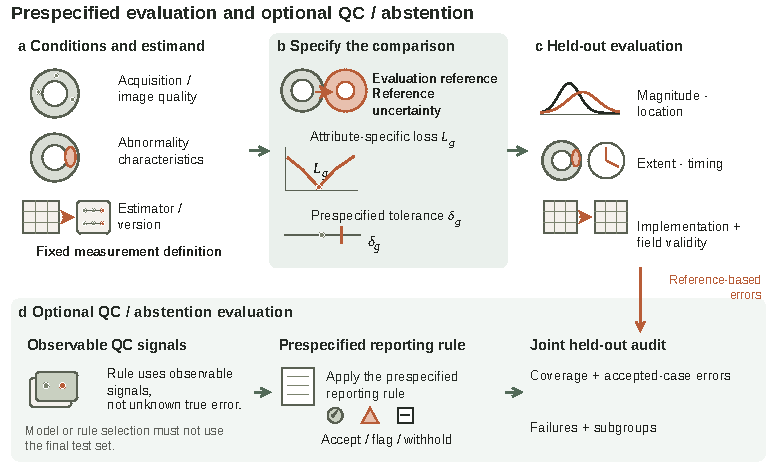
\includegraphics[width=\textwidth]{Figure_3_prespecified_evaluation.pdf}
\caption{Pre-specified evaluation for regional claims. Acquisition and abnormality conditions, estimator version and measurement definition are fixed before evaluation (a). The reference, attribute-specific loss and tolerance are declared (b). Results are reported separately for magnitude, location, extent, timing and mapping/field validity (c). Quality control or selective output is an optional implemented component; if used, its observable signals, coverage and accepted-case errors require audit (d). The figure is an original conceptual schematic and contains no study data. OpenAI Codex (gpt-5.6-sol) assisted deterministic Draw.io XML and Python-builder edits; no generative image model was used. Author verification is required before submission.}
\label{fig:evaluation}
\end{figure}

\subsection{Validation resources answer different parts of the question}\label{sec:resources}

No available resource simultaneously supplies routine cine, error-free dense in-vivo motion, broad pathology and unrestricted external testing. Their value lies in combination. STRAUS supplies controlled multimodal images and framewise reference meshes; the Stanford repository supplies human acquisitions with closely matched cine, DENSE and tagging locations; CMAC supplies a historical cross-method benchmark with sparse material-sensitive landmarks; and MRXCAT generations supply programmable motion and acquisition conditions. Their provenance and units of independence matter as much as file availability (\cref{tab:resources}).

STRAUS contains 18 \emph{virtual patients}, but these arise from three volunteer-derived multimodal templates, each driven through one healthy and five pathological electromechanical states (left bundle branch block, left-anterior-descending, left-circumflex and two right-coronary-artery ischaemia patterns), rather than 18 independent human anatomies. Each virtual case provides 3D cine MR, three tagged-MR orientations, ultrasound and framewise meshes; the paper used engineering strain for its regional curves\cite{zhou2018straus,strausdata}. The meshes therefore support known-correspondence displacement and strain calculations when coordinate system, reference frame, mesh identity and temporal sampling are matched. They do not reproduce the full distribution of human anatomy, disease, image artefact or model error.

The Stanford Cardiac Performance MRI resource has a different strength. Its laboratory page describes 51 healthy volunteers scanned at 3~T from 2023 to 2025, with whole-LV bSSFP cine and DENSE, tagging and mapping at specified corresponding locations\cite{stanforddata}. DataCite metadata updated on 27 July 2026 describes 55 participants---the same 51 healthy volunteers plus four people with aortic stenosis---under DOI 10.25740/xt223hz2438. These are versioned descriptions of one repository, not two cohorts. Neither total proves that every sequence is complete and usable for every participant, that all cine--DENSE slices are registered analysis pairs, or that a derived paper has an independent test cohort. DENSE magnitude and phase DICOMs also require reconstruction, phase unwrapping, displacement modelling, segmentation, spatial/temporal alignment and an explicit strain definition; they are material-sensitive observations, not error-free ready-made labels. No subject files were downloaded or processed for this review.

CMAC paired cine SSFP, 3D tagged MRI and 3D ultrasound from a dynamic phantom and 15 healthy volunteers. Its human reference comprised 12 landmarks (four walls at three LV levels) manually tracked by two observers in 3D tagging, with a reported median inter-observer variability of 0.84~mm\cite{tobongomez2013cmac,cmac2011}. This supports correspondence error at those landmarks and times, not dense strain accuracy between them. Original MRXCAT instead uses the XCAT phantom to generate cine or perfusion CMR with selectable cardiac/respiratory motion, sampling, coils and noise; the 2014 demonstration was primarily an acquisition/reconstruction simulator rather than a fixed disease cohort\cite{wissmann2014mrxcat}. MRXCAT2.0 adds statistical LV shape, biophysical healthy/infarct/dilated/hypertrophic function and generated tissue texture, exposing known simulated function for method testing\cite{mrxcat2023,mrxcat2repo}. It is a generator with exemplar outputs rather than a fixed number of independent participants.

Large multi-centre resources such as CMRxRecon2025 remain useful for reconstruction robustness and disease representation. Its official description covers multiple centres, scanners, disease groups and CMR contrasts, but does not establish tagging/DENSE motion labels or a fully paired cine--LGE cohort\cite{cmrxrecon2025official}. Segmentation collections and the Data Science Bowl similarly cannot be promoted to regional-motion references merely because they contain cine images. Detailed access, pairing, scale and uncertainty fields are provided in Supplementary Table~S2 and the editable resource table.

{\scriptsize\sloppy
\setlength{\tabcolsep}{2pt}
\begin{longtable}{L{0.12\textwidth}L{0.14\textwidth}L{0.18\textwidth}L{0.16\textwidth}L{0.20\textwidth}}
\caption{Complementary validation resources for cine-derived motion and strain. Counts denote the resource unit stated, not automatically independent test participants or complete paired analyses.}\label{tab:resources}\\
\toprule
Resource & Nature and scale & Available pairing/reference & What it can evaluate & Access and principal boundary \\
\midrule
\endfirsthead
\toprule
Resource & Nature and scale & Available pairing/reference & What it can evaluate & Access and principal boundary \\
\midrule
\endhead
STRAUS\cite{zhou2018straus,strausdata} & Synthetic; 18 virtual cases from 3 templates $\times$ 6 functional states & 3D cine, three tagged MR sequences and US with framewise VTK meshes & Dense correspondence, engineering strain, sampling and multimodal consistency in the simulated domain & Public, no login reported; only three source anatomies and imposed electromechanics/appearance \\
\addlinespace
Stanford Cardiac Performance MRI\cite{stanforddata} & Human; page: 51 healthy; DOI metadata: 55 total including 4 aortic stenosis & Whole-LV bSSFP cine; DENSE at matched locations; mid-LV tagging and other contrasts & In-vivo cross-sequence displacement/strain after explicit processing and alignment & Public repository, ODbL 1.0; completeness and usable pair count not yet file-verified \\
\addlinespace
CMAC\cite{tobongomez2013cmac,cmac2011} & Dynamic phantom and 15 healthy volunteers & Cine SSFP, 3D tagging and 3DUS; 12 manually tracked tagging landmarks & Sparse point correspondence and cross-modality benchmarking & Open access with attribution; sparse healthy reference, median inter-observer variability 0.84~mm \\
\addlinespace
MRXCAT\cite{wissmann2014mrxcat} & XCAT-based numerical generator, not a fixed human cohort & Prescribed anatomy/motion with cine/perfusion signal, coils, noise and sampling & Acquisition and reconstruction tests with known simulated motion & Code by non-commercial request; realism bounded by XCAT and signal assumptions \\
\addlinespace
MRXCAT2.0\cite{mrxcat2023,mrxcat2repo} & Generator for healthy, infarcted, dilated and hypertrophic LV cases & Shape model, biophysical simulation, texture and known functional values & Capacity and estimation error across generated anatomy and patho\-physiology & Public repository; generated instances are not independent clinical participants \\
\addlinespace
CMRxRecon 2025\cite{cmrxrecon2025official} & Multicentre, multivendor reconstruction resource with disease labels & Multiple CMR contrasts and reconstruction/QC material & Reconstruction robustness and domain shift & Challenge access terms; no declared dense motion truth or universal cine--LGE pairing \\
\bottomrule
\end{longtable}
}

\subsection{Reconstruction evidence is relevant but endpoint-specific}

Reconstruction changes the images supplied to a downstream estimator, and primary studies show both agreement and residual bias. REGAIN was trained on 1616 patients and tested prospectively in 181 participants; its paired breath-hold comparison used 94 patients and 36 healthy participants, while global radial, circumferential and longitudinal feature-tracking strain was available in 49 participants. Mean global-strain differences versus a separately acquired GRAPPA cine were near zero, but the 95\% limits of agreement remained \(-7\%\) to 6\% for radial, \(-2\%\) to 3\% for circumferential and \(-3\%\) to 3\% for longitudinal strain\cite{yoon2023regain}. CineVN compared prospectively accelerated acquisitions with conventional GRAPPA in 18 healthy volunteers. On individual mid-ventricular slices, CineVN had the smallest bias and narrowest limits among the tested accelerated reconstructions, yet all accelerated protocols significantly underestimated peak radial strain and overestimated peak circumferential strain; its 46-patient demonstration lacked a conventional reference and reported slice exclusions after segmentation failure\cite{vornehm2024cinevn}. These are measured reconstruction-plus-analysis results, not evidence that deep learning necessarily removes or preserves a focal abnormality.

Other designs bound the inference differently. In ten healthy volunteers, model-based deep-learning reconstruction improved the precision of global circumferential strain relative to compressed sensing at reduction factors 6 and 8 when full sampling was used as comparator, but circumferential bias and substantial radial underestimation remained and no regional lesion was tested\cite{tsuneta2025dlr}. DENT was developed from 5840 patients across nine centres and compared interpolated with acquired cine phases, including prospective image-quality comparisons in 49 patients and 12 healthy participants. It reported image-domain interpolation error and reader assessment, not myocardial strain or focal-abnormality recovery; even its deformation vectors were not validated as motion estimates\cite{morales2024dent}. Thus reconstruction and motion estimation should be evaluated jointly when the claim is regional, and any proposed mechanism---temporal smoothing, sharpening, alias suppression or hallucination---remains a hypothesis until tested against an attribute-appropriate reference.

\section{Reporting and interpretation in practice}

The consolidated reporting template is provided in Supplementary Note~5. Its essential logic is to identify the acquisition and reconstruction, estimator/version and interaction, complete strain estimand, statistical unit, validation target, failure policy and tested domain in the same record. For a focal claim, magnitude, location, extent and timing should be reported when each is relevant to the intended use; an attribute that was not inspected should not be relabelled as validated.

For clinical readers, a regional strain map should not be interpreted in isolation from the cine images, contours, tissue characterisation and global function. For technical readers, improving Dice, smoothness or Jacobian regularity is worthwhile but should be connected to the regional quantity that motivates the method. For both audiences, a negative result should identify which link failed: insufficient input cues, inadequate representation, failed estimation, mismatched strain definition, reference uncertainty or lack of clinical association.

Software clearance and commercial availability do not substitute for analytical validation of a specific regional output. Likewise, the existence of reference ranges does not make values interchangeable across products. Serial assessment is safest when acquisition, software, version and analysis conventions remain stable, while any change should be bridged empirically.

\section{Limitations of the evidence and of this review}

The evidence base is heterogeneous. Many studies are single-centre or use modest samples, healthy volunteers or a restricted disease spectrum. Paired DENSE/tagging studies face acquisition burden and alignment error. Commercial algorithms are not always described sufficiently to reproduce the exact mapping. Studies often report global or segmental peaks rather than the full field, and regional analyses may treat segments as independent. Publication bias may favour successful methods and well-behaved images.

This review used targeted rather than systematic searches, did not perform duplicate screening or risk-of-bias scoring, and did not pool effect sizes. Some recent 2026 method papers were available only at abstract or publisher-summary depth; they are used for publication status, design and high-level validation claims, not unreported numerical conclusions. Product and regulatory details were kept outside the central narrative because versions and indications change rapidly. The accompanying ledger records reading depth and unresolved items so that absence of inspection is not mistaken for absence of evidence.

The proposed attribute-based framework is an organising approach, not an established regulatory standard or new validated biomarker property. Tolerances must be justified for each intended use. No review can determine from published aggregate results whether a particular patient's regional map is correct.

\section{Conclusions}

Current evidence most directly supports cine-derived circumferential strain at whole-slice, global and AHA-segment scales when acquisition, software, myocardial layer, reference state and temporal endpoint are matched. Within those bounds, several paired studies found useful agreement with tagging or DENSE, and StrainNet improved end-systolic global and segmental Ecc agreement over the tested conventional feature-tracking pipeline. Scan--rescan and scar/outcome studies add evidence about precision and biological or prognostic relevance. They support use for their stated endpoints; they do not convert those endpoints into dense material-motion accuracy.

Support weakens as the requested output becomes more local or changes definition. Radial strain is consistently more product- and method-dependent. Basal/apical, endocardial/transmural, two-/three-dimensional, engineering/Green--Lagrange and end-systolic/peak values cannot be exchanged without qualification. The one independent prescribed-focal test retrieved, DeepStrain on MRXCAT2.0, found an attribute-specific result---circumferential strain preserved to within \(0.02\pm0.04\), radial strain underestimated in every case---from one scar geometry, one estimator and one slice position. In the studies reviewed, direct tests of focal abnormality centroid, lesion-boundary or width error, transmural extent recovery and peak-time error were uncommon or not reported; this is a statement about the inspected evidence, not proof that no such work exists. The observed differences in sampling, software and strain definition explain some discordance. Explanations based on information insufficiency, smoothing or low-dimensional bias remain hypotheses unless a study varies those factors or measures representation capacity directly.

A defensible regional claim should therefore name the acquisition, input, estimator, population, spatial unit, myocardial layer, reference state, time point, comparator and tolerance. Known-motion resources such as STRAUS and MRXCAT2.0 can test capacity and estimator error; CMAC contributes sparse cross-modality correspondence; and paired human cine--DENSE/tagging resources such as Stanford can test transfer only after explicit processing and alignment. Combining these complementary tests with participant-aware statistics and downstream clinical evaluation can identify where routine cine CMR preserves abnormality magnitude, location, extent and timing---and where the appropriate conclusion remains unresolved.


\section*{Declarations}

\subsection*{Ethics approval and consent to participate}
Not applicable. This review did not collect new participant data.

\subsection*{Consent for publication}
Not applicable to the review content. The corresponding author must confirm that all author and institutional details are approved before submission.

\subsection*{Availability of data and materials}
No new participant dataset was created. The review is based on published sources. The accompanying author-review package contains the search record, evidence ledger, figure sources and reproducible manuscript source; these audit materials are not intended to imply that the review was systematic.

\subsection*{Competing interests}
\textbf{Author confirmation required before submission.} This draft does not certify the absence or presence of competing interests.

\subsection*{Funding}
\textbf{Author confirmation required before submission.} No funding statement has been certified for this draft.

\subsection*{Author contributions}
The current title page lists Ziying Huo as the sole author. Authorship, order and contribution wording must be confirmed against the journal's criteria before submission. No contribution by a supervisor or other person is inferred from background materials.

\subsection*{Acknowledgements}
\textbf{Author confirmation required before submission.} Names, contributions and permission to acknowledge individuals must be confirmed by the author.

\subsection*{Declaration of generative AI and AI-assisted technologies in the manuscript preparation process}
OpenAI Codex was used to assist with targeted literature-query preparation, bibliographic and source checks, evidence structuring, manuscript and table revision, language editing, LaTeX preparation and deterministic quality assurance. Claude Code (Anthropic) was subsequently used to merge the v8.1 and v9 drafts, restore the method-lineage and prescribed-focal-test content and their previously verified references, add cross-references and Supplementary Table S3, and run LaTeX, BibTeX and static consistency checks. No raw cardiac images were processed and no new experimental result was generated. All figures in this revision were inherited byte-for-byte from the selected v8.1 baseline and were not created or edited in the v9 or merge tasks; their existing captions retain the earlier production disclosure. The corresponding author must review and verify all content, citations, figures and declarations, confirm the journal's live policy interpretation and accept responsibility before submission; that review is not asserted here.

\subsection*{Figure provenance and permissions}
The retained explanatory figures and graphical abstract are inherited from the selected v8.1 package. Their file hashes are reported before and after revision and are identical; no image pixels, internal text, layout or editable source were changed in v9. No patient image, published result trace or identified third-party artwork appears in the retained visible figures. This production record does not certify authorship, originality, publication rights or journal-policy acceptance. The corresponding author must inspect the figures and graphical abstract, confirm their scientific content and rights, and decide whether the graphical abstract requires prior editorial clarification.

\setlength{\bibsep}{2pt}
\bibliographystyle{jcmr-review}
\bibliography{references}

\end{document}
